
\section{OpenLearning}
\subsection{Overview}
OpenLearning is a ASX listed company that provides an LMS for educational providers. It was founded by Adam Brino, Richard Buckland (COMP6441 lecturer) and David Collien and is used in security courses at UNSW.\\
It works with universities such as UNSW and Taylor's University (based in Malaysia) to deliver MOOCs (massive open online courses). It also features an LMS that educational institutions can use. Some courses at UNSW currently use it such as COMP6441 (Security), and many universities such as UNSW, UTS, ACU, Charles Sturt University and more also use the platform.\\
Unlike other content management systems such as Moodle, OpenLearning is not free or open source and can be quite costly.\\

\subsection{Home}
When logged in, the home page of OpenLearning is quite confusing.\\
\begin{figure}[h!]
    \centering
    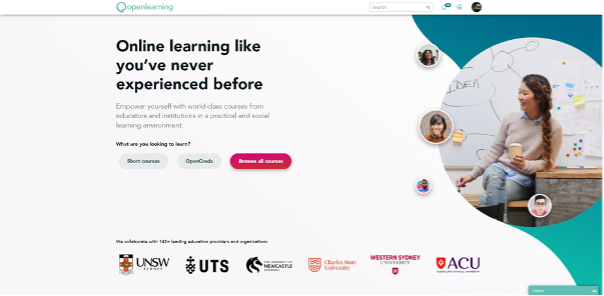
\includegraphics[scale=0.4]{openlearning-homepage}
    \caption{OpenLearning Homepage}
\end{figure}

For students, it can be quite confusing how to reach their courses. The home page clearly directs you to search for a new course offered by OpenLearning, not a course you are already enrolled in. \\
\\
The balloon icon in the top right should be clicked to reach my courses. \\
\begin{figure}[h!]
    \centering
    
\includegraphics[scale=0.4]{openlearning-balloon}
    \caption{This icon is confusing and it is not clear how to get to my educational resources.}
\end{figure}

\subsection{Course Home Page}
\begin{figure}[h!]
    \centering
    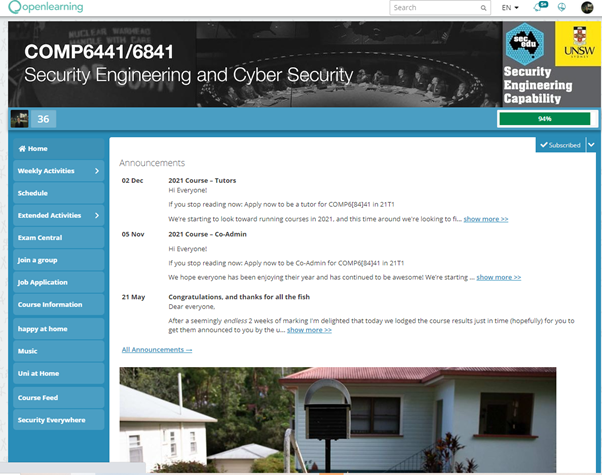
\includegraphics[scale=0.4]{openlearning-coursehome}
    \caption{OpenLearning Course Home}
\end{figure}
The course home page UI is good, with clear links to information and important announcements being easily viewable.\\

\subsection{Performance}
\begin{figure}[h!]
    \centering
    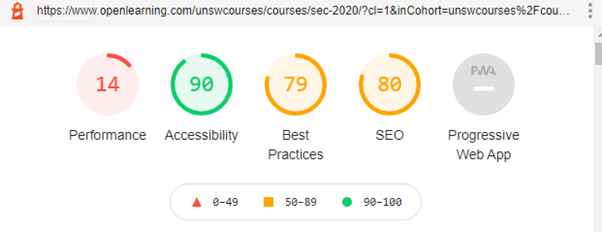
\includegraphics[scale=0.4]{openlearning-lighthouse}
    \caption{Google Lighthouse Result}
\end{figure}
The overall performance of OpenLearning is poor, with pages feeling slow and sluggish with Google Lighthouse, a performance testing tool, giving 14/100 for performance. However, accessibility seems otherwise quite good, with a 90/100 score. \\

\subsection{Forum and Commenting}
\begin{figure}[h!]
    \centering
    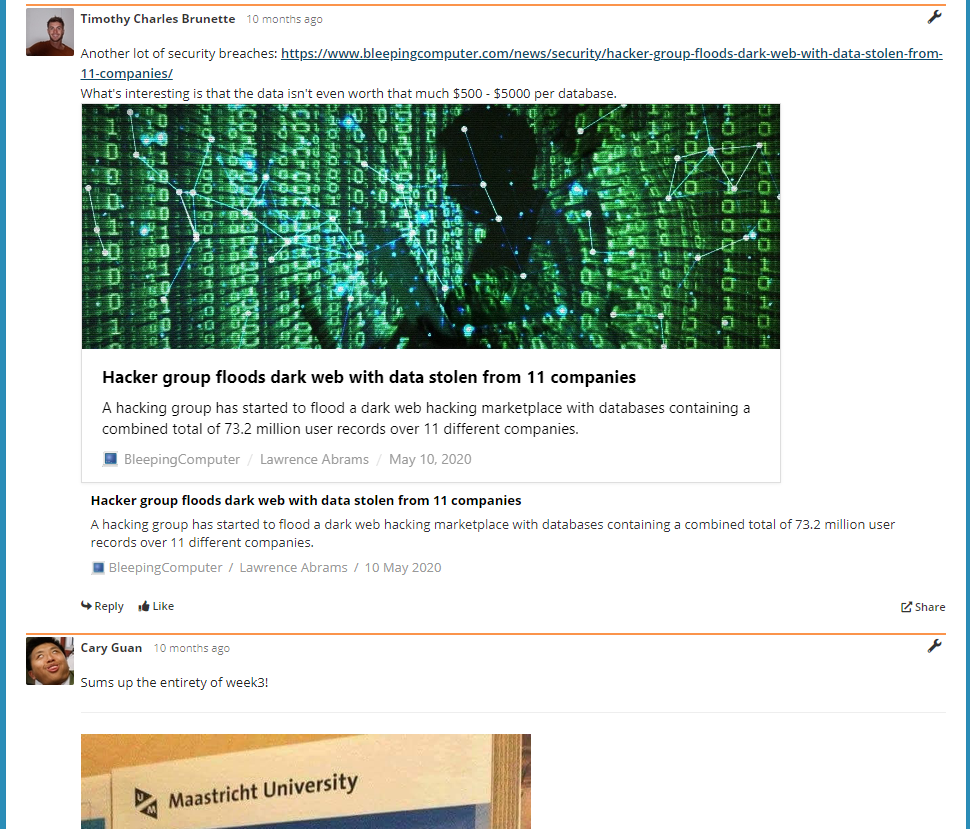
\includegraphics[scale=0.4]{openlearning-forums}
    \caption{OpenLearning comments system}
\end{figure}
OpenLearning makes it quite difficult to communicate with other students, with a comment feature available but not searchable or sortable at all. There does not seem to be a forum feature either, and so in courses such as COMP6441, it can be very difficult to collaborate and communicate with classmates. \\


\subsection{Data Migration}
\begin{figure}[h!]
    \centering
    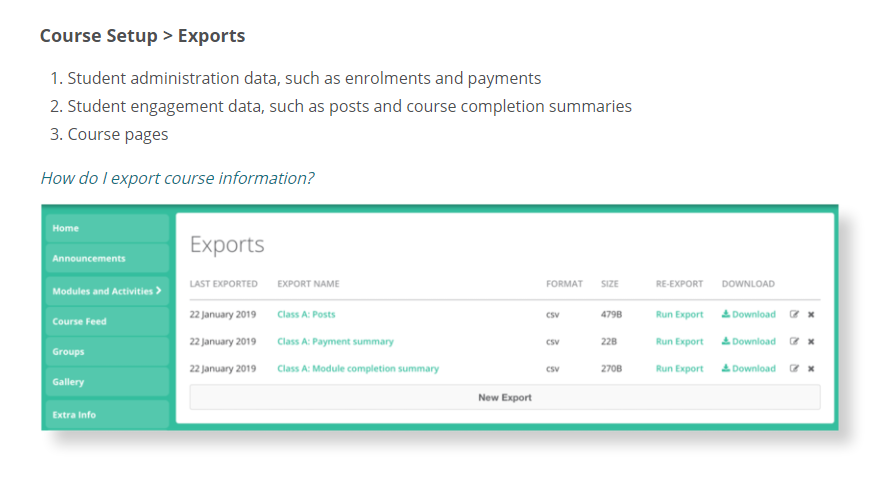
\includegraphics[scale=0.4]{openlearning-export}
    \caption{Exporting data in OpenLearning}
\end{figure}
Data migration seems quite poor in OpenLearning. There are no support articles available on how to import data from another course, and so it seems quite difficult to create a new course. There is a basic system to export data into a csv file, but there does not seem to be a way to import data either.

\subsection{Conclusion}
OpenLearning is a good platform for instructors and students, with a huge feature set with blogs, commenting, and a very flexible course setup. However, the UI, performance and stability can be significantly improved to be more competitive with other CMS platforms. A searchable forum can also be implemented, and little data migration features can hinder courses that use the platform, as time is wasted uploading and curating content for courses.

